\documentclass[a4paper]{article}

\usepackage{cmap}
\usepackage[T2A]{fontenc}
\usepackage[utf8]{inputenc}
\usepackage[english, russian]{babel}
\usepackage{amsmath, amsfonts, amssymb, amsthm, mathtools}
\usepackage{fullpage}
\usepackage{url}
%\usepackage{indentfirst}

\usepackage{todonotes}

\usepackage{cite}
\usepackage{csquotes}

\usepackage{tikz}

\usepackage{graphicx}
\graphicspath{{img/}}

\title{Компьютерные сети}
\author{Мельников С.А.}
\date{12/07/2021}

\begin{document}

\maketitle
\tableofcontents
\newpage

%%% Переопределение списков на приближенные к технической документации
\renewcommand{\labelenumii}{\theenumi.\arabic{enumii}}	\renewcommand{\labelenumiii}{\labelenumii.\arabic{enumiii}}

\section{О курсе}
Автор курса -- Алексей Степченко, имеет опыт работа сетевым администратором, а также сетевым инженером

Регламент курса:
\begin{itemize}
	\item 8 вебинаров по 2 часа 
	\item Видеозаписи
	\item Домашние задания
	\item Консультации по вопросам
\end{itemize}

Необходимый софт:
\begin{itemize}
	\item Cisco Packet Tracer
\end{itemize}

Не смотря на название курса, для карьерной траектории системным администратором, необходимо дополнительно знать такие темы, как:
\begin{itemize}
	\item Системное администрирование
	\item Поддержка пользователей
\end{itemize}

Среди навыков и типовых задач системного администратора на начальном уровне можно отметить: 
\begin{itemize}
	\item Поднять сервер
	\item Обмен файлами через сервер
	\item Настройка создания и хранения бекапов
	\item Поднять домен Windows
	\item Настроить маршрутизатор
	\item Поднять Git-сервер
\end{itemize}

Полученные знания на курсе являются достаточно ценными, т.к. их не знает 80~\% системных администраторов

Зачем программисту знать, как работают сетевые технологии?
\begin{itemize}
	\item Масштабирование приложений
	\item Производительность приложения
	\item Безопасность приложения
\end{itemize}

У любого ИТ-специалиста должна присутствовать теоретическая база:
\begin{itemize}
	\item Устройством компьютера 
	\item Сетевые технологии
	\item Аппаратное обеспечение
	\item Сетевое обеспечение
\end{itemize}

Цели курса:
\begin{itemize}
	\item Изучение основных концепций сетевых технологий (системные знания о работе сетей)
	\item Настройка сетевых протоколов (настройка сетей)
	\item Разработка архитектуры небольших сетей (проектирование сетей)
	\item Диагностика сети
	\item Изучение работы протоколов верхних уровней
\end{itemize}

Все сетевое взаимодействие можно разбить на несколько абстрактных уровней, изучение предлагается от низшего (физического) уровня к более высоким

План курса:
\begin{enumerate}
	\item Урок 1. Основы компьютерных сетей. Технология Ethernet. Часть 1 (Настройка физического уровня)
	\item Урок 2. Физический и канальный уровни. Технология Ethernet. Часть 2 (Настройка канального уровня)
	\item Урок 3. Сетевой уровень Часть 1 (Настройка сетевого уровня)
	\item Урок 4. Сетевой уровень Часть 1 (Настройка сетевого уровня)
	\item Урок 5. Транспортный уровень (Настройка транспортного уровня)
	\item Урок 6. Углубленное изучение сетевых технологий. Часть 1 (Настройка сетевых служб)
	\item Урок 7. Углубленное изучение сетевых технологий. Часть 2 (Настройка сетевых служб)
	\item Урок 8. Прикладной уровень. Перспективные сетевые технологии (Анализ HTTP-трафика)
\end{enumerate}

\section{Урок 1. Основы компьютерных сетей. Технология Ethernet. Часть 1}
В уроке будут рассмотрены следующие темы:
\begin{itemize}
	\item Основные концепции сетей передачи данных
	\item Эталонная модель OSI/ISO и стек протоколов TCP/IP
	\item Введение в технологию Ethernet
	\item Диагностика физического уровня
\end{itemize}

\textbf{Назначение компьютерных сетей} --- передача информации между различными сетевыми устройствами, в том числе компьютерами. 

Самая известная сеть на сегодняшний день --- интернет. Интернет (глобальная сеть, WAN)--- всемирная система объединенных компьютерных сетей для хранения и передачи информации

Сеть построена на базе стека протоколов TCP/IP
Предоставляет сервисы:
\begin{enumerate}
	\item World Wide Web (WWW)
	\item Социальные сети
	\item Почта
	\item Обмен файлами и др.
\end{enumerate}

\subsection{Основные понятия}
\subsubsection{Виды связей}
\begin{itemize}
	\item Simplex --- односторонняя связь, передача в одну сторону (рис.\ref{fig:pic-1}) \\ Примеры: 
		\begin{itemize}
			\item Теле/радио-вещание
			\item Передача сигнала от спутников GPS
		\end{itemize}
		\begin{figure}[!h]
			\centering
			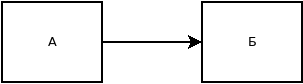
\includegraphics[width=5cm]{1-simplex.png}
			\caption{Пример обмена сообщениями в виде связи Simplex}
			\label{fig:pic-1}
		\end{figure}
	\item Half-duplex --- двусторонняя связь, но в один момент времени может передавать только одно устройство (по очереди)(рис.\ref{fig:pic-2}) \\ Примеры:
		\begin{itemize}
			\item Общение по рации, когда можно слушать канал, либо, нажав на кнопку, передавать в него
		\end{itemize}
		\begin{figure}[!h]
			\centering
			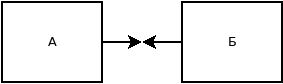
\includegraphics[width=5cm]{2-half-duplex.png}
			\caption{Пример обмена сообщениями в виде связи Hald-duplex}
			\label{fig:pic-2}
		\end{figure}
	\item Full-duplex или просто Duplex --- двусторонняя передача, оба устройства могут одновременно вести передачу (рис.\ref{fig:pic-3}) \\ Пример:
		\begin{itemize}
			\item Разговор по телефону
		\end{itemize}
		\begin{figure}[!h]
			\centering
			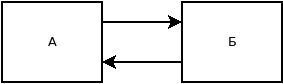
\includegraphics[width=5cm]{3-full-duplex.png}
			\caption{Пример обмена сообщениями в виде связи Full-duplex}
			\label{fig:pic-3}
		\end{figure}
\end{itemize}

В сетях используются все 3 вида связи

\subsubsection{Методы передачи данных (типы адресации)}
\begin{itemize}
	\item Unicast --- передача единственному (одному) адресату (\ref{fig:pic-4})
	\begin{figure}[!h]
		\centering
		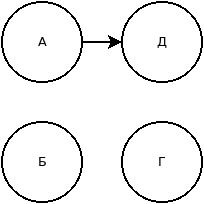
\includegraphics[width=4cm]{4-unicast.png}
		\caption{Пример типа адресации Unicast}
		\label{fig:pic-4}
	\end{figure}
	\item Broadcast --- широковещательная передача данных всем устройствам (всем кто их слышит) (\ref{fig:pic-5})
	\begin{figure}[!h]
		\centering
		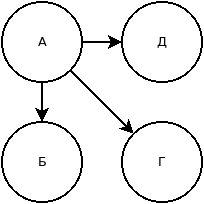
\includegraphics[width=4cm]{5-broadcast.png}
		\caption{Пример типа адресации Broadcast}
		\label{fig:pic-5}
	\end{figure}
	\item Multicast --- передача данных в группе устройств (\ref{fig:pic-6})
	\begin{figure}[!h]
		\centering
		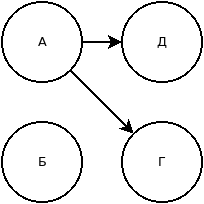
\includegraphics[width=4cm]{6-multicast.png}
		\caption{Пример типа адресации Multicast}
		\label{fig:pic-6}
	\end{figure}
\end{itemize}

\subsection{Виды коммутации}
\subsubsection{Коммутация каналов}
Первая концепция при разработке сетей --- коммутация каналов. Т.е. в сети с коммутацией каналов между 2-мя конечными устройствами устанавливается физический канала. Пример: телефонная сеть

Концепция заключается в использовании связей между различными АТС и возможности установления связи между конечными устройствами при наличии физических связей между АТС абонентов. Пример присоединения устройства А и Б представлен на рисунке \ref{fig:pic-7-channel-commutation}

\begin{figure}[!h]
	\centering
	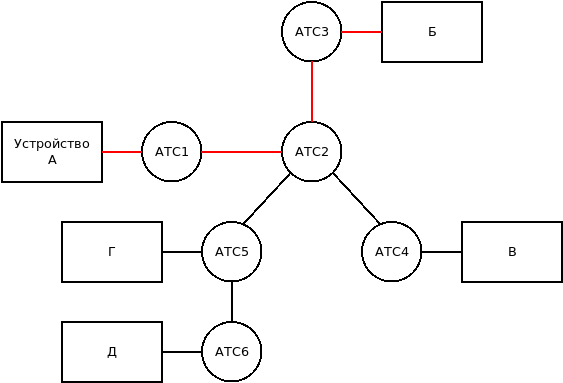
\includegraphics[width=10cm]{7-channel-commutation.png}
	\caption{Коммутация каналов}
	\label{fig:pic-7-channel-commutation}
\end{figure}

Основной минус подхода заключается в ограниченности физических связей между различными АТС, т.е. при отсутствии физической связи между АТС2 и АТС4, абонент устройства Б не сможет связаться с абонентом В. Также каждый контакт с другим устройством требует отдельного канала от устройства до АТС. Т.е. пользователю устройства А потребуется 4 канала до АТС и наличие связей от своей АТС к другим АТС, а также наличие каналов для устройства А на стороне других пользователей, чтобы иметь возможность независимого общения со всеми пользователями

Преимущество: стабильность соединения, т.к. используется заранее определенный физический канал с определенным набором характеристик. Нет конфликтов и помех

\subsubsection{Коммутация пакетов}
В сети с коммутацией пакетов информация от каждого устройства делится на небольшие пакеты, и данные передаются по одним и тем же физическим каналам. Пример: компьютерные сети

\begin{figure}[!h]
	\centering
	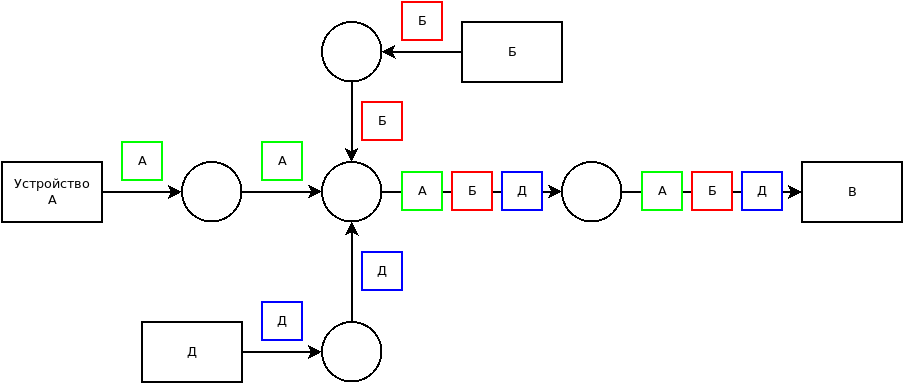
\includegraphics[width=\textwidth]{8-package-commutation.png}
	\caption{Коммутация пакетов}
	\label{fig:pic-8-package-commutation}
\end{figure}

Концепция: вместо установки отдельных физических каналов для каждого отдельного получателя, сделали 1 общий физический канал и сделали общую очередь для всех сообщений другим абонентам, которая последовательно передается другим получателям

На примере рис.\ref{fig:pic-8-package-commutation}, видно, как устройство B может получить пакеты от 3 остальных устройств в рамках очереди по 1 физическому каналу

Однако требуется отдельная система распределения пакетов адресатам для обеспечения корректной работы

Наряду с преимуществами, есть минус: нет гарантированной пропускной способности канала. Т.е. мы не можем гарантировать абоненту А, что его пакет будет доходить до абонента В с определенной скоростью, так как не знаем количество других пакетов на этом участкей

\subsection{Классификация сетей}
\subsubsection{По размеру}
Сети можно классифицировать по географическому размеру (рис.\ref{fig:pic-9-geo-network-types}):
\begin{itemize}
	\item WAN (wide area network) --- глобальная вычислительная сеть, наш интернет
	\item MAN (metropolian area network) --- вычислительная сеть города (опционально)
	\item LAN (local area network) --- локальная вычислительная сеть, небольшая сеть с покрытием 1-2 домов
\end{itemize}

\begin{figure}[!h]
	\centering
	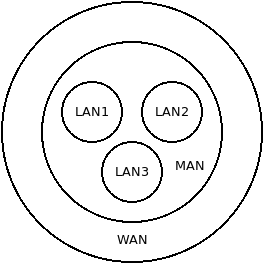
\includegraphics[width=5cm]{9-geo-network-types}
	\caption{Классификация сетей по географическому размеру}
	\label{fig:pic-9-geo-network-types}
\end{figure}

Соответственно глобально, весь интернет, вся всемирная паутина состоит из городских сетей (провайдеры), которые состоят из локальных сетей, за которыми уже закрепляются конкретные пользователи. Есть и просто отдельные локальные сети

\subsubsection{Виды топологий}
\textbf{Сетевая топология} --- это структура графа (схема сети, чертеж), на вершинах которого находятся конченые узлы сети (компьютеры/телефоны/принтеры) и сетевое оборудование (коммутаторы, роутеры), а ребра --- физические линии связи между узлами

Сетевые топологии могут быть:
\begin{itemize}
	\item Физическими --- определяет как физически соединены устройства в сети (как соединены устройства)
	\item Логическими --- определяет направления потоков данных между узлами сети и способы передачи данных (как внутри идут данные)
\end{itemize}

С помощью различных сетевых технологий (например WLAN), можно очень хитро организовать логическую топологию, которая на физический даже близко не будет похожа

Существует набор уже готовых шаблонов подобных схем (рис.\ref{fig:pic-10-topology-types})
\begin{figure}[!h]
	\centering
	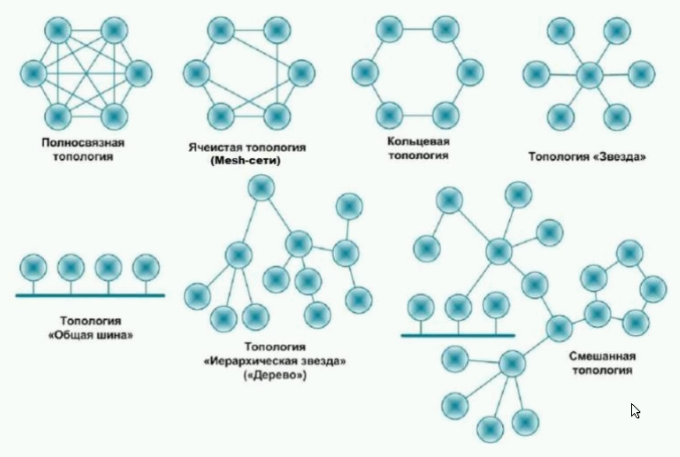
\includegraphics[width=\textwidth]{10-topology-types}
	\caption{Виды топологий}
	\label{fig:pic-10-topology-types}
\end{figure}

Виды топологий:
\begin{itemize}
	\item \textbf{Общая шина}, где есть 1 шина к которой подключаются все устройства, при этом все устройства конфликтуют за среду передачи данных (по такому принципу был сделан первый Ethernet)
	\item \textbf{Звезда}, есть некоторое звено посередине к которому подключены все остальные устройства
	\item \textbf{Кольцевая}, когда все устройства обмениваются данными по кольцу
	\item \textbf{Полносвязная} (Full-mesh), есть некоторое количество устройств, которые все связаны друг с другом
	\item \textbf{Ячеистая} (Mesh-сети), также является примером Mesh-сетей, как и Full-mesh, но без некоторых связей
	\item \textbf{Иерархическая звезда} (Дерево), является примером связанных между собой топологий <<Звезда>>. Часто когда строят сети, их называют древовидной, потому что закладываются определенные принципы деления звеньев (какие то отвечают за доступ клиентам, другие за коммутацию высокоскоростного трафика) и делят их на слои (access layer, distribution layer, core layer и др.)
\end{itemize}

В жизни редко используют чистые типы топологий и создает смешанные топологии, решающие определенные задачи

\subsection{Абстракции для описания сетевого взаимодействия}
Реализацию коммутации пакетов можно реализовать различными способами:
\begin{itemize}
	\item Разные способы адресации
	\item Способы разделения и сборки
	\item И др
\end{itemize}

При этом система должна быть гибкой и масштабируемой (развитие без ограничения архитектурой)

Существуют 2 основные сетевые модели стеков протоколов, описывающие работу сетей передачи данных:
\begin{itemize}
	\item \textbf{Модель OSI} (Open System Interconnection), она же \textbf{эталонная модель взаимодействия открытых систем} (ЭМВОС) --- это 7-ми уровневая абстрактная модель, разработанная Международной Организацией по Стандартам (International Organization for Standardization - ISO)
	\item \textbf{Стек протоколов TCP/IP} --- 4-ех уровневая модель, разработанная по инициативе Министерства обороны США. Используется сейчас, как основной стек протоколов в сетях (промышленный стандарт), где TCP и IP являются основными протоколами в стеке
\end{itemize}

Но часто для обозначения уровней используется используется OSI, где обозначен физический уровень для работы с сетевым оборудованием, а дальнейшую разработку уже ведут по протоколу TCP/IP, т.к. он проще. Обе являются теоретическими моделями

\subsubsection{Соответствие уровней модели OSI и стека TCP/IP}
Модель призвана все сетевое взаимодействие поделим на слои, где каждый слой будет решать свою задачу (рис.\ref{fig:pic-11-tcpip-vs-osi})

\begin{figure}[!h]
	\centering
	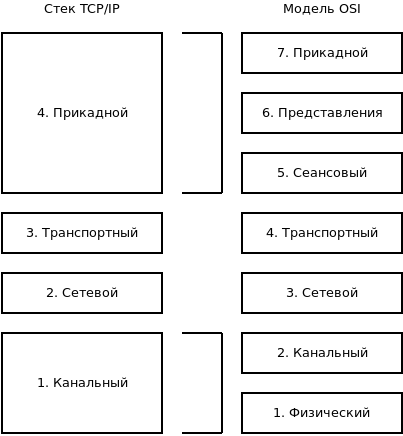
\includegraphics[width=10cm]{11-tcpip-vs-osi}
	\caption{Соответствие уровней модели OSI и стека TCP/IP}
	\label{fig:pic-11-tcpip-vs-osi}
\end{figure}

Уровни модели OSI:
\begin{enumerate}
	\item \textbf{Физический} --- набор стандартов, которые описывают непосредственно среду передачи данных (кабели, количество жил, диаметр жил, коннекторы, разъемы, напряжения, формы сигналов и т.д). Пример: витая пара --- одна технология физического уровня, wi-fi другая технология
	\item \textbf{Канальный} --- программный уровень (внутри сетевой карты), решает вопрос доступа к среде передачи данных (т.е. к Физическому уровню). Соответственно в зависимости от используемых на Физическом уровне технологий, требуются определенные технологии на канальном уровне, чтобы читать пакеты с витой пары или, например, стандарт wi-fi канального уровня 
	\item \textbf{Сетевой} --- уровень, который должен обеспечить универсальную адресацию по всей планете и обеспечить доставку информации по адресу. Т.е. сетевой уровень использует IP-адресацию (глобальная адресация) и задача сетевого уровня доставить определенный пакет определенному получателю (маршрутизация, адреса пакетов)
	\item \textbf{Транспортный} --- большой объем информации организуется на небольшие пакеты, которые на транспортном уровне на одном конце разбивает большой файла на кусочки, на другом конце его собирает обратно в целое
	\item \textbf{Сеансовый} --- установка/прекращение соединения (соединение --- логическое, абстрактное понятие, сессия обмена данными между устройствами), проверка корректности доставки
	\item \textbf{Представления} --- отображение данные, шифровка/расшифровка, конвертация, изменения кодировки и т.д.
	\item \textbf{Прикладной} --- произвольное формирование неких данных, приложение формирует данные, которые передаются по следующим уровням и до адресата они должны дойти так, как они и передавались (например, формирование сообщения в чате и его восприятие адресатом)
\end{enumerate}

Уровни стека TCP/IP
\begin{enumerate}
	\item Канальный --- 
	\item Сетевой
	\item Транспортный --- работает протокол TCP, который отвечает за разбивку на кусочки, доставку и повторную доставку
	\item Прикладной 
\end{enumerate}

Основное отличие стека TCP/IP от OSI заключается в его простоте. Однако большой минус стека TCP/IP в его Канальном уровне, где объединены Канальный и Физический (как у модели OSI), что накладывает определенные трудности

Основной стек по которому работает современный интернет --- стек TCP/IP. Но в последнее время сетевые инженеры чаще используют модель OSI (в основном 1,2,3,4 и 7 уровни), т.к. по этим уровням очень хорошо классифицируется сетевое железо

\subsection{Стек TCP/IP}
\begin{enumerate}
	\item \textbf{Канальный уровень} (Link Layer) отвечает за доступ к физической среде и за саму передачу в физической среде \\
	Единица информации: Фреймы \\
	Технологии: Ethernet 
	\item \textbf{Сетевой уровень} (Internet Layer) отвечает за адресацию, доставку пакетов адресату \\
	Единица информации: Пакеты \\
	Протокол: IP
	\item \textbf{Транспортный уровень} (Transport Layer) разбивка потока данных и собирает в другом месте\\
	Единица информации: Сегменты \\
	Протокол: TCP, UDP
	\item \textbf{Прикладной уровень} (Application Layer) формирует поток данных \\
	Единица информации: Потоки данных \\
	Протокол: HTTP, SSH, DNS, DHCP и множество других
\end{enumerate}

\subsubsection{Инкапсуляция}
Инкапсуляция --- процесс упаковывания поля данных в протокол в соответствии с положением процесса иерархии уровней стека 

Рассмотрим процесс на примере обмена сообщением между ПК1 и ПК2 (рис.\ref{fig:pic-12-tcpip-incapsulation})
\begin{enumerate}
	\item \textbf{Прикладной уровень ПК1}, задача сгенировать поток данных на уровне приложения (Application Data)
	\item Далее поток данных передается на \textbf{Транспортный уровень ПК1}. Соответственно Транспортный уровень разбивает поток данных на кусочки (Data 1) в зависимости от протокола и добавляет Заголовок (Header) Транспортного уровня (H3 + Data 1), что вместе является сегментом. H3 может содержать данные об адресации, портах, необходимая для Транспортного уровня
	\item Далее сегмент данных передается на \textbf{Сетевой уровень ПК1}(Протокол Транспортного уровня инкапсулируется в протокол Сетевого уровня), который к сегменту (H3 + Data 1) и добавляет свой Заголовок (H2) и формирует, тем самым пакет. H2 - содержит информацию, которая необходима для корректной обработки Сетевым уровнем на стороне ПК2
	\item После пакет передается на \textbf{Канальный уровень ПК1}(Сетевой инкапсулируется в Канальный), ((Data 1 + H3) + H2), которому присваивается Заголовок Канального уровня (H1), содержащий служебную информацию для корректной обработки на Канальному уровне ПК2 и формируется фрейм
\end{enumerate}

\begin{figure}[!h]
	\centering
	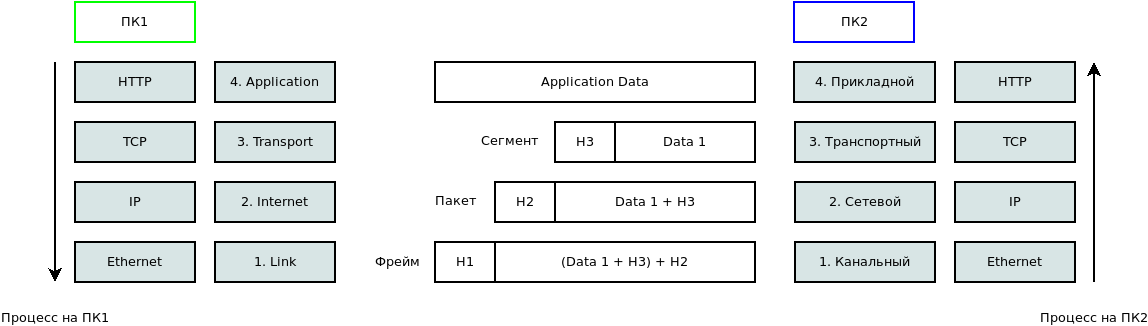
\includegraphics[width=\textwidth]{12-tcpip-incapsulation}
	\caption{Инкапсуляция в стеке TCP/IP}
	\label{fig:pic-12-tcpip-incapsulation}
\end{figure}

\subsubsection{Декапсуляция}
В целом отрабатывает алгоритм Инкапсуляции, но в обратном порядке:
\begin{enumerate}
	\item \textbf{Канальный уровень ПК 2} получил Фрейм. После прочтения H1, если фрейм соответствует Канальному уровню ПК, запускается алгоритм Декапсуляции: анализирует какому верхнему уровню (протоколу) отдать, стирает Заголовок H1 и осуществляет передачу
	\item \textbf{Сетевой уровень ПК 2} читает Заголовок H2 пакета, адресованному ему, читает какому протоколу его передать и стирает Заголовок H2, осуществляет передачу
	\item \textbf{Транспортный уровень ПК2} читает заголовок H3 сегмента, читает, анализирует и передает на Прикладной уровень
	\item \textbf{Прикладной уровень ПК2} получает и отображает данные пользователю в режиме Приложения
\end{enumerate}

Такой порядок осуществляется в случае использования аналогичных протоколов, а вместе с тем и технологий у ПК1/ПК2. В реальной же жизни существуют устройства, которые позволяет переключать технологии, например Switch, у которого и точка доступа и Ethernet-интерфейс и его задачей будет являться адаптировать фрейм под соответствующий протокол

\subsection{Сетевая технология Ethernet}
Часто протоколы физического и канального уровня тесно связаны и использование определенной канальной технологии определяет технологии физического уровня

\textbf{Ethernet} --- семейство технологий пакетной передачи данных в компьютерных сетях, использующих метод множественного доступа с контролем несущей и обнаружения коллизий - CSMA/CD 

Название Ethernet (буквально <<эфирная сеть>> или <<среда сети>>) связано с тем, что первоначально принцип работы этой технологии был заимствован из радио технологии ALOHAnet

Ethernet описывается стандартами группы IEEE 802.3 (номер спецификации)

Ethernet сейчас является одной из самый распространенных технологий ЛВС. В середине 90-х, он вытеснил такие сетевые технологии, как ARCNET и Token Ring

\subsubsection{Основы Ethernet}
Первой физической схемой подключения (физической топологией) Ethernet была <<Шина>> (рис.\ref{fig:pic-13-tcpip-first-version})

Особенности:
\begin{itemize}
	\item Все устройства конфликтуют за среду передачи данных
	\item Передача ведется в режиме half-duplex на скорости до 10 Мбит/сек
	\item Технологии имели название 10BASE5 и 10BASE2 (первые цифры обозначают скорость в Мбит/сек, BASE означает работу без несущей (позже изменилось), 2/5 максимальная длина соединительного кабеля (в 100 метрах, т.е. 10BASE5 максимальная длина 500 м))
	\item Использовался коаксиальный кабель и Т-образный разъем для подключения устройств
	\item На концах кабелей необходимо было иметь специальный устройства, терминаторы, иначе сигнал отражался и приводил к <<падению>> сети
	\item При этом при разрыве какой-либо части, ложится весь сегмент
\end{itemize}

\begin{figure}[!h]
	\centering
	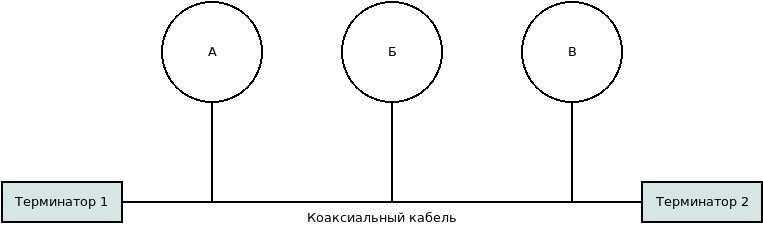
\includegraphics[width=15cm]{13-tcpip-first-version}
	\caption{Основы Ethernet}
	\label{fig:pic-13-tcpip-first-version}
\end{figure}

\subsubsection{Коаксиальный кабель}
Коаксиальный кабель представлен на схеме (рис.\ref{fig:pic-14-coaxial-cabel})

Кабеля были:
\begin{itemize}
	\item С тонким коаксиалом
	\item С толстым коаксиалом, можно было использовать на более больших дистанциях
\end{itemize}

Устройство:
\begin{itemize}
	\item Центральная жила
	\item Диэлектрик
	\item Экранирующая оплетка
	\item Внешняя изоляция
\end{itemize}

Коаксиальный кабель имеет 2-контакта: центральную жилу и экранирующую оплетку, т.е. 1 пара

\begin{figure}[!h]
	\centering
	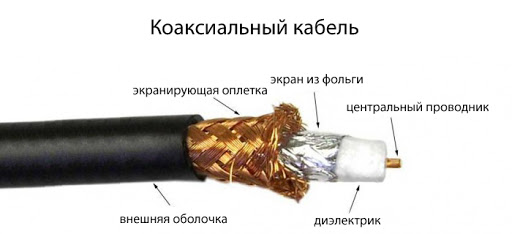
\includegraphics[width=15cm]{14-coaxial-cabel}
	\caption{Коаксиальный кабель}
	\label{fig:pic-14-coaxial-cabel}
\end{figure}

Передача без несущей означает отсутствие сигналов в эфире передачи по умолчанию. Если идет передача данных она передается в эфир и ее слышит конечное устройство

Однако использование передачи без несущей не всегда бывает применим, например в радиопередаче передача звука не возможна без несущей, т.к. радиоволны обладают колебаниями другой частоты (выше чем звуковые). Соответственно для их передачи от антенны до антенны передается несущий сигнал (частота), она не имеет полезной нагрузки, но используется как основа для передачи полезного сигнала с помощью различных методов, модуляции, изменения частоты, высоты импульсов и т.д. На другом же конце такой сигнал демодулируется и получается исходных сигнал. Например радио работает благодаря несущей и радиомодуляции

Несущий сигнал использует ту частоту, которая может с нормальным качеством перейти через требуемую среду

\subsubsection{Проблемы ранних Ethernet}
\begin{itemize}
	\item Режим half-duplex. Устройство не может одновременно вести прием и передачу
	\item Обрыв кабеля выводил из строя всю сеть
	\item Неудобства при работе с коаксиальным кабелем 
\end{itemize}

\subsubsection{Переход на витую пару со сменой топологии на звезду}
\textbf{Hub (концентратор)} --- сетевое устройство, работающее на первом уровне модели OSI (рис.\ref{fig:pic-15-ethernet-hub})

Любой фрейм, прошедший на порт хаба, дублируется на все его порты кроме того, с которого он этот фрейм получил. 10BASE-T (T -- twisted, витая пара)

\begin{figure}[!h]
	\centering
	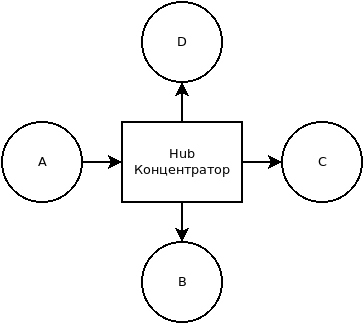
\includegraphics[width=7cm]{15-ethernet-hub}
	\caption{Использование hub в раннем Ethernet}
	\label{fig:pic-15-ethernet-hub}
\end{figure}

Отличия от решения на основе топологии <<Шина>>:
\begin{itemize}
	\item Поменяли кабель с коаксиального на витую пару. В витой паре уже несколько жил (количество жил взяли с запасом)
	\item Начали использовать концетратор (Hub), к нему были подключены все компьютеры. К нему приходит фрейм на порт и он передается одновременно на все (без каких-либо дополнительных коммутаций и задержек)
\end{itemize}

Пример такого устройства (рис.\ref{fig:pic-16-ethernet-hub}):
\begin{figure}[!h]
	\centering
	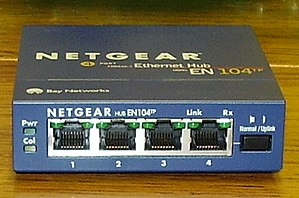
\includegraphics[width=10cm]{16-ethernet-hub}
	\caption{Пример реального hub}
	\label{fig:pic-16-ethernet-hub}
\end{figure}

А также пример такой схемы, показывающая ее пассивность (рис.\ref{fig:pic-17-ethernet-hub-schema}):
\begin{figure}[!h]
	\centering
	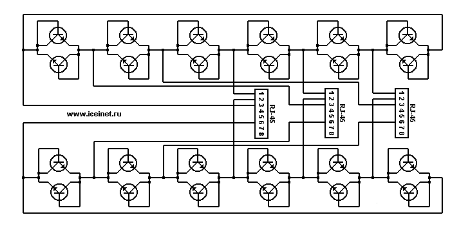
\includegraphics[width=\textwidth]{17-ethernet-hub-schema}
	\caption{Электрическая схема реального hub}
	\label{fig:pic-17-ethernet-hub-schema}
\end{figure}

\subsection{Витая пара и ее особенности}
Работа хаба и соответственно витой пары определяется его разъемом, коннектором RJ-45 (8P8C)(рис.\ref{fig:pic-18-ethernet-rj-45}). RJ - сокращение от \textsc{registered jack}
\begin{figure}[!h]
	\centering
	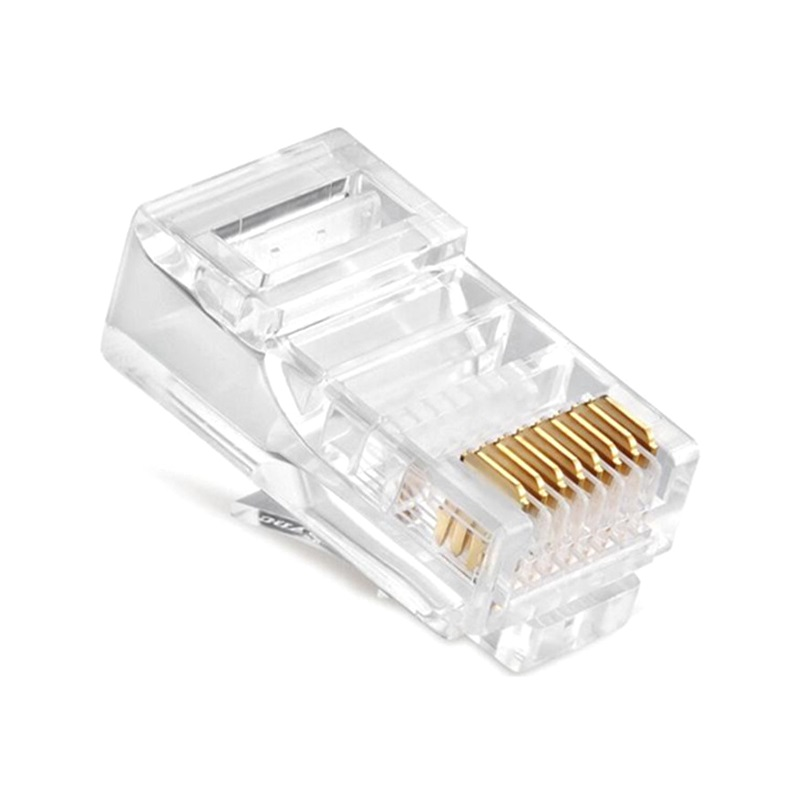
\includegraphics[width=5cm]{18-ethernet-rj-45}
	\caption{Коннектор 8P8C (RJ-45)}
	\label{fig:pic-18-ethernet-rj-45}
\end{figure}

Сам кабель <<витая пара>>, получил такое название благодаря специфике организации жил (рис.\ref{fig:pic-19-ethernet-twisted-pair})
\begin{figure}[!h]
	\centering
	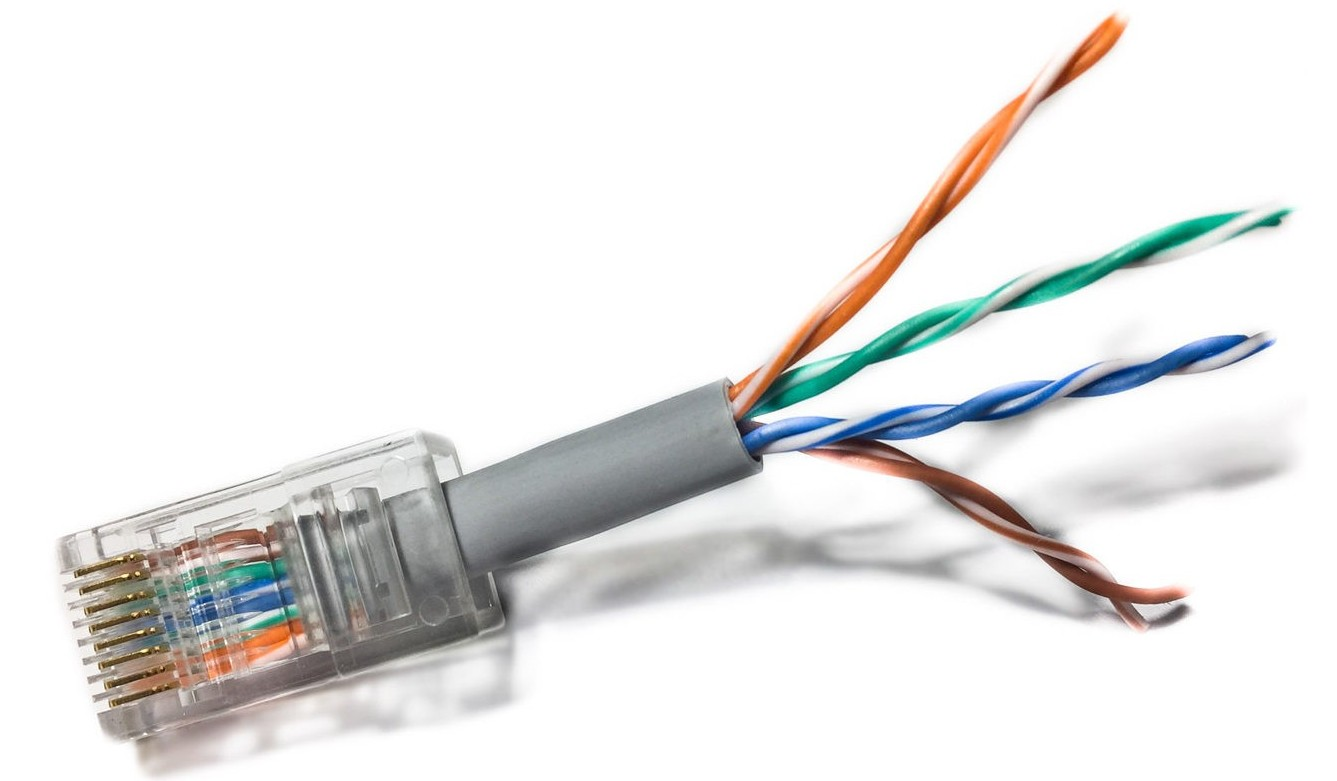
\includegraphics[width=7cm]{19-ethernet-twisted-pair}
	\caption{Устройство <<Витой пары>>}
	\label{fig:pic-19-ethernet-twisted-pair}
\end{figure}

Особенности витой пары:
\begin{itemize}
	\item Завиты они для погашения наводки (электро-магнитных помех, помехозащищенность)
	\item Витые пары бывают 2-ух парники и 4-ех парники
	\item Для сетей со скоростью 10 Мбит/сек и 100 Мбит/сек достаточно 2-ух пар, для 1 Гбит/сек необходимо 4-пары
	\item Кабели делятся по категориям и определяют характеристики кабеля
	\item Самая распространенная категория 5E для современных Ethernet и самый распростаненный тип витой пары UTP (unshielded twisted pair)(неэкранированная витая пара, пластиковая оплетка и 2/4 витых пары)
	\item В ряде случаев применяют экранированные витые пары (у них есть оплетка, фольга), обычно для связи между домами. Однако данный вид кабелей требует другой вид коннекторов, экранированных (рис.\ref{fig:pic-20-ethernet-rj-45-ftp})
	\item Существует отличие патч-кордов от кабелей, продаваемых в бухте и заключается оно в количестве жил. Поставляемые кабели в бухтах для прокладки одножильные, они надежные, но плохо гнутся, соответственно при частых механических воздействиях (перестановка) высока вероятность его перелома. Короткие патч-корды же делаются из многожильных проводов, они легко гнутся и более живучие
	\item Существует также и отличие коннекторов для одножильных и многожильных проводов и они разные 
\end{itemize}

\begin{figure}[!h]
	\centering
	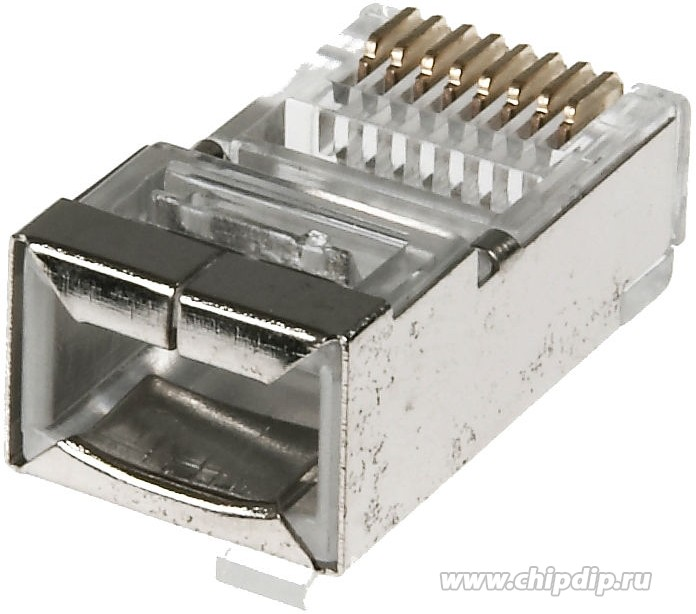
\includegraphics[width=5cm]{20-ethernet-rj-45-ftp}
	\caption{<<Витая пара>> экранированная}
	\label{fig:pic-20-ethernet-rj-45-ftp}
\end{figure}

\subsubsection{Обжимка витой пары}
Существует 2 основных стандарта обжимки:
\begin{itemize}
	\item Прямой кабель
	\item Перекрестный кабель (кросс)
\end{itemize}

\begin{figure}[!h]
	\centering
	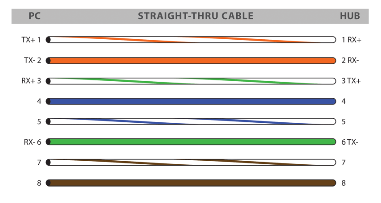
\includegraphics[width=10cm]{21-straight-thru-cable}
	\caption{Прямая обжимка}
	\label{fig:pic-21-straight-thru-cable}
\end{figure}

\begin{figure}[!h]
	\centering
	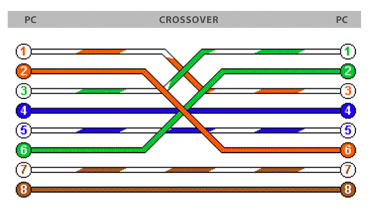
\includegraphics[width=10cm]{22-crossover-cable}
	\caption{Перекрестная обжимка}
	\label{fig:pic-22-crossover-cable}
\end{figure}

Каждый из них имеет свои правила обжимки и их применение обусловлена назначением использования. Если рассмотреть это на примере раннего Ethernet, и возьмем кросс-обжимку (где меняется 1 и 3 пара). Зеленая пара используется для передачи данных (tx, transmit), оранжевая для приема данных (rx, receive). Если устройство старое, то она не умеет автоматически определять и будет передавать по нужным кабелям. Соответственно мы просто соединяем tx-выходы (для передачи) c rx-выходами (для получения) другой стороны, чтобы осуществить корректный обмен информацией (в противном случае оба устройства будут передавать в rx-группу, и получать из tx-группы, обмена не будет). Этот нюанс был особенно актуален раньше, т.к. сетевые карты не имели алгоритмов автоматической распиновки

Также актуально правил, что при подключении разных устройств (например ПК и хаб) мы используем прямую распиновку, если соединяем однородные устройства (например хаб и хаб), то нужна кросс-распиновка

На сегодняшний день в 99~\% используется прямая распиновка, соответственно подключение можно пробовать по нему, если же все-таки попалось устройство с кросс-пиновкой, используем соответствующий кабель

Синий и коричневый кабеля в 10/100 Мбит/сек и Ethernet не используется, однако в 1 Гбит/сек будут задействованы все 4 пары и только прямая обжимка

\subsubsection{Основные протоколы семейства Ethernet, работающие по витой паре}
\begin{itemize}
	\item \textbf{10BASE-T} или просто Ethernet. Скорость 10 Мбит/с, Half/Full Duplex. Используется 2 пары
	\item \textbf{100BASE-T} или Fast Ethernet. Скорость 100 Мбит/с, Hald/Full Duplex. Используется 2 пары
	\item \textbf{1000BASET-T} или Gigabit Ethernet. Скорость 1000 Мбит/с, \textbf{только} Full-Duplex. Используется 4 пары, каждая из которых работает в режиме Full Duplex, 4 пары по 250 Мбит/сек
	\item Для всех стандартов можно применять витую пару UTP (unshielded twisted pair - неэкранированная витая пара) категории 5е. У всех стандартов ограничение по длине 1 кабеля -- 100 м (в силу уменьшения помехозащищенности, сеть может просто не работать)
	\item Все эти протоколы поддерживают обратную совместимость (если сетевое устройство поддерживает Fast Ethernet -- это значит, что оно гарантированно поддерживает и Fast Ethernet и Ethernet и т.д.)
	\item Большинство устройств поддерживает авто-согласования скорости и по режиме Duplex (если мы соединениям 2 устройства, то возможно создание сети с характеристиками самого худшего устройства с точки зрения его протокола, т.е. если соединить 10BASE-T и 1000BASE-T устройства, то станет возможным поднять сеть на 10Мбит/с)
\end{itemize}

В интерфейсе Windows
2:00:00






\newpage
\section{Дополнительная информация}
Оптоволокно имеет определенное преимущество перед медью, это длина возможной связи при максимальной скорости (например с помощью оптоволокна можно подключить достаточно удаленные объекты с приемлемой скоростью передачи пакетов)

Full-duplex, как вид связи можно реализовать на 1 жиле, т.е. не нужно 2 жил для обеспечения одновременной двусторонней передачи

ADSL --- технология использует уплотнение сигналов, создавая целый спектр несущих частот, которые уже модулируются полезным сигналом



\section{Дополнительное задание}
\begin{itemize}
	\item Почитать про физику передачи данных через кабели
	\item Физика процессов передачи данных по витой паре
\end{itemize}

\section{Литература}
\begin{enumerate}
	\item Методические материалы: \url{https://docs.google.com/document/d/18J6-ld0mUPM6UJ4VVosYIDIk2X_BBRgZVrGwrgqLt4A/edit#heading=h.uvp6qax5r1ok}
	\item Презентация: \url{https://docs.google.com/document/d/18J6-ld0mUPM6UJ4VVosYIDIk2X_BBRgZVrGwrgqLt4A/edit#heading=h.uvp6qax5r1ok}
\end{enumerate}


\end{document}